\chapter{Problem Analysis and Solution Design}
\section{Problem Definition}
\subsection*{CROs and DSOs}

Oscilloscopes available in secondary schools or sixth forms are generally basic
analogue oscilloscopes known as CROs, or Cathode Ray Oscilooscopes (named so
because the display is a Cathode Ray Tube).~\autocite{DoctronicsScopes}

The alternative is a DSO, or Digital Storage Oscilloscope. These work in a very
different way to CROs. Like in a CRO, the input signal is first passed through
some analogue circuitry to amplify it, and so on. However, it's then sampled
into a digital signal using a DAC (Digital to Analogue Converter) and processed
using a microcontroller (perhaps using the help of an FPGA\fdeffpga or a
DSP\fdef{Digital Signal Processor}{a custom microcontroller especially designed
  to perform various \textit{signal processing} functions (e.g., performing a
Discrete Fourier Transform to obtain the frequency spectrum of a signal, or
using Principal Component Analysis to seperate two audio signals)}), before
being output onto some sort of digital screen.~\autocite{TiePieScopes}

\subsection*{Advantages of DSOs}

DSOs offer a number of advantages over CROs. As well as relatively basic
differences such as the traces being much more sharply defined, DSOs allow
digital signal processing to be done on the input signal. This means that, for
example, DFTs (Discrete Fourier Transforms)\footnote{While DFTs are the ones
  most famous transformations, mainly due to the prevalence of the FFT (Fast
  Fourier Transform) algorithm, in practice DCTs (Discrete Cosine Transforms)
  are more commonly used as they can be calculated quicker to achieve a similar
end effect} can be run to produce a frequency spectrum of the input signal,
allowing the user to see both time-domain and frequency-domain representations
of the signal.\footnote{This also means that DSOs can be used as basic spectrum
analysers: essentially devices that plot frequency spectrums, these have uses as
far ranging as determining GSM interference when planning mobile phone networks}

Additionally, a DSO can be used to create a basic Logic Analyser. This is
essentially the digital equivalent to an oscilloscope --- a relatively large
number of digital wires and buses are connected to the Logic Analyser and a
timing diagram is output\footnote{In more advanced, standalone Logic Analysers,
more complicated outputs such as decoded Ethernet packets can be
output}.~\autocite{ElectronicDesignMSO}

\begin{figure}
  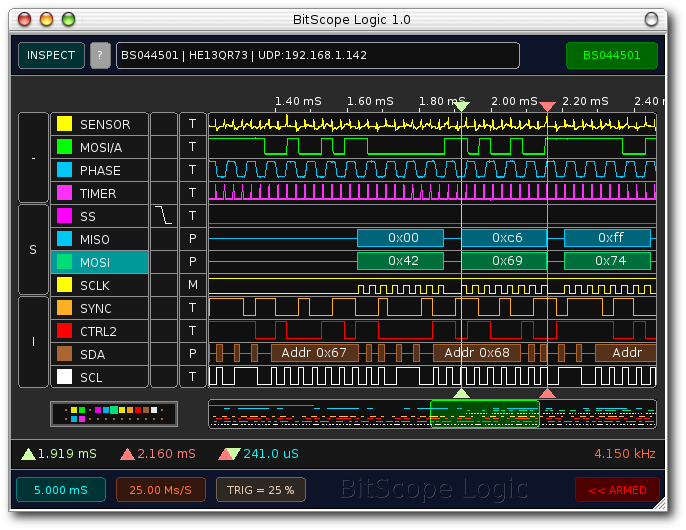
\includegraphics[width=\linewidth]{img/bitscope.png}
  \caption[Logic Analyser Example Output]{Example output from a Logic Analyser ~\autocite{fig:Bitscope}}
\end{figure}

\subsection*{Problem Definition}

This project aims to create a Digital Sampling Oscilloscope, with the following
more advanced features included:

\begin{itemize}
  \item Frequency spectrums of the input signals available
  \item Basic capability as a Logic Analyser
\end{itemize}

From now on, oscilloscope will be used to refer to a Digital Sampling
Oscilloscope and CRO will be used to explicitly refer to a Cathode Ray
Oscilloscope.

\section{Research into Existing Oscilloscopes}

Using two articles from \Citeauthor{PicotechScopes}\autocite{PicotechScopes} and
\Citeauthor{GabotronicsScopes}\autocite{GabotronicsScopes}, digital
oscilloscopes can be categorised by the following criteria:

\begin{itemize}

  \item \textbf{Bandwidth} The bandwidth\footnote{Most commonly, bandwidth is
      taken to be the range of fraquencies where the signal has an amplitude
      gain of $\SI{-3}{\dB}\approx 71\%$} in \SI{}{\Hz} of the initial analogue
      stages of the oscilloscope. Common values range from \SI{100}{\kHz} to
      \SI{100}{\MHz}.

  \item \textbf{Type of Sampling} There are two common types of sampling,
    real-time and equivalent-time sampling. With real-time sampling the scope
    samples sequentially over the wave, whereas with equivalent-time sampling
    the scope captures a sample from a different part of the wave every time
    period. This is perhaps illustrated more clearly
    in~\cref{fig:EquivalentTimeSampling}.

  While equivalent-time sampling offers a much faster sampling rate, it is more
  complicated to implement so for the purposes of this project we will only be
  considering real-time sampling.

  \item \textbf{Sample Rate} The rate (in \SI{}{\Hz} or the equivalent
  \textit{samples per second}) at which the oscilloscope can take individual
  digital samples from the signal. Common values range from \SI{10}{\kHz} to
  \SI{1}{\GHz}.

  \item \textbf{Resolution} The number of bits each sample has. Common values
  are 8, 12 and 16 bits. This determines the precision of the oscilloscope, and
  hence the minimum noise.

  \item \textbf{Memory Depth} The number of samples the oscilloscope can store
  at one time. Measured in either words, or bits (for example, if the resolution
  is 8 bits then a depth of 128 words is equivalent to 1024 bits). Intuitively,
  this can be thought of as the horizontal resolution. Common values range from
  100 samples to \SI{10}{M} samples.

  \item \textbf{Triggers Available} The different options to trigger the
    oscilloscope to start capturing samples, with the most common one being edge
    triggering \autocite{PicotechTriggers} (when the signal passes a threshold
    on a rising edge\footnote{A falling edge could also be used, but the type of
    edge is part of the trigger specifications and stays constant}). There are
    also more advanced triggers such as pulse width triggering, which triggers
    the scope when a digital pulse of a certain width is detected. Some
    expensive oscilloscopes can provide extremely complicated triggers: e.g.,
    decoding Ethernet, TCP/IP\footnote{The protocol used for internet
    networking} and HTTP\footnote{The protocol used to transfer web pages over
    the internet} packets from a digial input, and eventually triggering the
    analogue inputs when a certain webpage is requested.

  \item \textbf{Input range} The minimum and maximum range of input voltages
    that can be detected by the oscilloscope. A typical value would be from
    \SI{\pm 50}{\mV} to \SI{\pm 50}{\V}. In many cases, this will be a
    relatively small range, but an active scope probe (a test probe with an
    amplifier inside it) will be used to broaden this range.

\end{itemize}

\begin{figure}
  \centering
  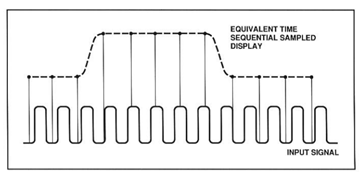
\includegraphics{img/equivalent_time_sampling.png}
  \label{fig:EquivalentTimeSampling}
  \caption[Equivalent Time Sampling Diagram]{Diagram illustrating equivalent time sampling ~\autocite{fig:EquivalentTimeSampling}}
\end{figure}

\section{Practical Investigations}

\subsection{Breadboard Frequency Investigation}

A limiting factor in the bandwidth and sampling rate\footnote{The sampling rate
will be influenced by this much more than one would expect --- for example, with
the MAX114 ADC, to capture samples at \SI{1}{\MHz} the ADC must be communicated
with at \SI{15}{\MHz}~\autocite{MAX114}} will be due to stray capacitances and
inductances on the breadboards\footnote{As detailed later on, a PCB will be used
for the final system, however prototyping will occur on breadboards so the
maximum frequency on a breadboard is still a limiting factor} used to construct
the system, which will cause a great deal of noise at high frequencies.

Because of this, the first practical investigation undertaken was to find the
attenuation of a signal running through a breadboard at various frequencies.

A signal generator was connected to an oscilloscope through a number of
connections on a breadboard, and the amplitude of the final signal recorded at
various frequencies. The same experiment was then repeated connecting the
oscilloscope directly to the signal generator.

For each frequency, the gain in \SI{}{\dB} was then calculated using the
equation

\begin{align*}
\text{Gain} & = 10\log_{10}\left(\frac{P_{out}}{P_{in}}\right)\\
            & = 10\log_{10}\left[\frac{\frac{\left(V_{out}\right)^2}{R_{out}}}{\frac{\left(V_{in}\right)^2}{R_{in}}}\right]\\
            & \approx 10\log_{10}\left[\frac{\left(V_{out}\right)^2}{\left(V_{in}\right)^2}\right]\\
            & = 20\log_{10}\left(\frac{V_{out}}{V_{in}}\right)
\end{align*}

\fxwarning{Photos and results}

\subsection{Oscilloscope Reliability Investigation}

An existing oscilloscope (in this case, a CRO) will be a vital part of testing
the osilloscope, so it would be wise to test it's accuracy first.

An FPGA\fdeffpga was programmed to produce a square wave at a number of
different frequencies, and the wave was looked at on an oscilloscope. Due to
their completely different nature compared to microcontrollers, FPGAs are
usually programmed in a language called Verilog. While the details are beyond
the scope of this project\footnote{\textcite{VerilogTutorial}, found online at
\url{http://www.asic-world.com/verilog/index.html}, is an excellent resource for
learning Verilog}, let us just say that Verilog is a way of describing the
propogation of signals based on dependencies on both time and other
signals\autocite{VerilogWiki}.

The FPGA was programmed to perform a 50\% duty-cycle clock divisions of the
FPGA's internal\footnote{A high-quality crystal oscillator} \SI{50}{\MHz} clock,
meaning the output frequency could be easily calculated using

\begin{equation*}
  f = \frac{\SI{50}{\MHz}}{2^n}
\end{equation*}

where $n$ is the clock divisor.

\fxwarning{Photos and results}
\fxwarning{Verilog code}

\section{Numerical Parameters}

\subsection*{Frequency and Sampling Rate}

The sampling rate should be as high as feasibly possible to allow the
oscilloscope a wide variety of uses. By \textcite{ShanonNyquist}, the maximum
frequency\footnote{Actually, that's the maximum sinusoidal frequency that we can
sample. By Fourier, all other waveforms can be represented as a sum of
sinusoids, and in reality sampling at 25 times the frequency of the waveform
means that we'll be able to get a high enough amount of detail for most
non-sinusoidal waveforms} that we can sample is half the sampling rate. In
reality, because of the basic real-time sampling method being used it must be at
the very least 25 times less than the sampling rate (allowing just over 12
samples for each half-period of the wave).

ADCs in a DIP\footnote{Electronics components come in a variety of different
packages of many different shapes and sizes. Generally, those that fit in a
breadboard are part of the DIP (dual in-line package) family: e.g., CDIP
(Ceramic DIP) and PDIP (Plastic DIP). Other packages, such as TSOP, are usually
much smaller and suitable only for soldering onto PCBs. While a PCB will be used
for the final oscilloscope, soldering surface-mount chips (a generic term for
all packages smaller than DIP, such as TSOP) requires unavailable specialist
equipment.} package (suitable for breadboards) are not readily available beyond
\SI{2}{\MHz}. Furthermore, the only \SI{2}{\MHz} DIP ADC, the AD7822, is
renowned for being particularly difficult to interface with a microcontroller.
Instead, an ADC with a maximum sampling rate of \SI{1}{\MHz} will be used (many
DIP ICs can provide this sampling rate).

However, at such a high speed getting the full sampling rate out of an ADC is
not usually possible with a microcontroller (because, for example, a control bit
might have to go high then low again for \SI{20}{\ns}, but a microcontroller
with a \SI{16}{\MHz} clock can only do this in an absolute minimum of
\SI{62.5}{\ns}). So the oscilloscope sampling rate will be specified as at least
\SI{500}{\kHz}.

This means the maximum frequency that should be sampled is
$\frac{\SI{500}{\kHz}}{25} = \SI{20}{\kHz}$.

\subsection*{Bandwidth}

The maximum frequency into the analogue amplification stage will be
\SI{20}{\kHz}, but we also need to take into consideration harmonics (remember,
by Fourier any non-sinusoidal signal can be represented as a sum of sinusoidal
signals of increasing frequency). To be safe, we will specify a minimum
bandwidth of \SI{1}{\MHz}.

\subsection*{Resolution}

Inaccuracies in the oscilliscope output are more likely to be caused by the
analogue circuitry (in particular, the digital potentiometers are only accurate
to 0.25\%) than a low resolution, so an 8 bit resolution will suffice (this
offers an accuracy of $\approx 0.4\%$, more accurate than the digital
potentiometer accuracy). This also means ADCs will be more readily available, as
8 bit DIP ADCs are more common than higher resolution ones.

\subsection*{Memory Depth}

The memory depth needs to be large enough to have a horizontally precise signal,
but small enough that the samples can easily be stored in the microcontroller.
For these reasons, 1024 words (equivalent to 8192 bits or \SI{1}{\kilo\byte}
with an 8 bit resolution) will be chosen. Most microcontrollers have multiple
\SI{}{\kilo\byte} of RAM, so multiple signals can easily be stored in the
RAM.

\subsection*{Input Range}

For the minimum input range, we'll choose the standard \SI{\pm 50}{\mV}, however
high-bandwidth rail-to-rail op amps are only cheaply available up to \SI{\pm
5}{\V} so for the maximum input range we'll choose \SI{\pm 5}{\V}\footnote{While
  the input to the op amp could be a higher voltage than the supply voltage, a
digital potentiometer will be needed to automatically adjust the gain of the op
amp. These only work up to to the supply voltage.}.

\subsection*{Triggers Available}

For the purposes of this project, simple edge triggering will more than suffice.
Both the channel on which and the threshold at which the trigger occurs will be
adjustable by the user.

\section{Communication with Android Device}
\label{sec:CommOptions}

As detailed in ~\cref{sec:user_interface}, an Android device will be used as the
frontend to the oscilloscope. This means that the microcontroller must somehow
communicate with the device.

There are 4 feasible ways that this could be achieved: via WiFi, Bluetooth and
USB.

\subsection*{USB}

This would perhaps be the easiest way to implement the communication. Small
discrete devices, such as the CP2102~\autocite{CP2102}, convert between the
relatively complicated USB protocol and the simple UART protocol. In fact,
nearly all microcontrollers now come with a built-in USART interface, so the
microcontroller side of things would be literally `plug and
play'\footnote{Various configuration words would have to be moved to registers
to initialise USART communication at the start of the program, but beyond that
there would simply be registers for writing data, reading data and checking if
data is available to be read}.

On the Android side, the microcontroller would appear as a serial communication
device. The `usb-serial-for-android' library~\autocite{AndroidUSBSerial} would
make it trivial to communicate with the microcontroller from an Android
application via a serial port\footnote{Serial ports are a throwback to the times
when computers had physical RS232 serial connections, over which data could be
sent and received using a very simple protocol. Nowadays, serial ports are
virtual ports that send and receive data over much more complicated protocols
such as USB and Bluetooth.}.

Because the connection is wired, there would be minimal interference so the
speed could potentially go as high as the maximum USB 2.0 bit rate\footnote{Baud
rate figures are not officially available, but it's clear from the bit rate that
it would be extremely high} of \SI{480}{\mega\bit\per\second}.

However, there would be a major disadvantage to this approach: that the
oscilloscope would have to be physically connected to the tablet. This means the
tablet would not be able to be freely moved around while using the oscilloscope.
While a traditional oscilloscope operates this way, allowing wireless connection
would make the oscilloscope much more vertasile: for example, the relatively
cheap oscilloscope hardware could be left permanently connected in a
hard-to-access electronics project, and accessed wirelessly when needed through
the Android tablet.

\subsection*{WiFi}

It would be far beyond the scope of this project to communicate just using a
\SI{2.4}{\GHz} antenna, so instead a discrete WiFi module would be needed. These
have traditionally been relatively expensive\footnote{So much so that for a time
in the mid-2000s it become very common for devices such as amateur robots to
communicate with computers over the \SI{2.4}{\GHz} spectrum, but using a
different protocol to WiFi. This author has not been able to find out why such
devices were significantly cheaper than WiFi devices, but one suspects it is due
to both the complexity of the WiFi protocol and licensing costs required to
implement it.}, however Texas Instruments has recently released the CC3000, a
module much cheaper than the competition.~\autocite{CC3000Cheap}

If the initial project was being created on a custom PCB, then the CC3000 could
simply be included as a component on the PCB. However, the prototype is being
created on a breadboard, so a breakout board (a board that contains the CC3000
and an antenna and exposes a digital interface to the CC3000 via pins that can
fit in a breadboard) is needed.

The cheapest, most widely available breakout board is Adafruit's `Adafruit
CC3000 WiFi Breakout with Onboard Ceramic Antenna`. Adafruit are a US-based
company, but the board can be easily obtained in the UK via eBay. However, it
costs \pounds 25.

In terms of complexity, using the CC3000 would be more complicated than using
USB, but not insurmountably so. Libraries exist for both AVR and PIC
microcontrollers to interface with the CC3000, and on the Android side it would
simply require interfacing with a TCP socket\footnote{Again, TCP sockets are
significantly outside the scope of this project, but they can essentially be
thought of as virtual counterparts to physical sockets. A wire can be used to
connect physical sockets together to allow communication between them, and a
protocol such as TCP (the base protocol for the internet) does the same thing
for virtual sockets.} (not significantly more complex than communicating via a
USB serial connection).

One advantage WiFi has over USB is that it offers a wireless connection,
negating the main disadvantage of USB. In addition, it would be able to offer
very fast data transfer rates like USB (also like USB, official baud rate
figures are not available, but the latest standard\footnote{802.11n, which is
supported by most wifi devices nowadays} offers a bit rate of up to
\SI{600}{\mega\bit\per\second}).

However, the main disadvantage is the price. Even with the CC3000, the cheapest
available option, at \pounds 25 the WiFi module would make up a considerable
amount of the total cost of the oscilloscope.

\subsection*{Bluetooth}

Like with WiFi, discrete Bluetooth modules are readily available. These operate
in a similar way to the USB CP2102 --- the microcontroller communicates with the
module via USART, and the Android device via a serial port.

One example of such a module would be a JY-MCU HC-06. Via eBay, these are
available relatively cheaply (about \pounds 5).

This means one key advantage of Bluetooth is simplicity. The inbuilt USART
functionality of the microcontroller can be used on the microcontroller side,
and a Bluetooth serial library used on the Android side. The heavy lifting of
the Bluetooth communication is done by the HC-06 and software built into the
Android device.

Bluetooth obviously offers a wirelesss connection, and should work up to about
\SI{10}{\m}. The maximum baud rate supported is
\SI{1.3824}{\mega\bit\per\second}, which is slower than both USB and WiFi but
fast enough for our purposes (remember the oscilloscope takes 8-bit samples at
\SI{500}{\kHz} so the sampling rate is only \SI{4}{\mega\bit\per\second}).

\subsection*{Chosen Solution}
The required wired connection between the oscilloscope and Android device ruled
out USB, leaving WiFi and Bluetooth.

Data transfer speeds are not a big issue in this use case, and Bluetooth's
\SI{1.3824}{\mega\bit\per\second} is certainly fast enough. This means the key
differences between Bluetooth and WiFi are complexity and cost. Bluetooth wins
both of these, so Bluetooth was chosen as the communication method between
microcontroller and Android device.
